Exercise 2 addresses implementing a parallel algorithm for blurring images.
The original image, which is used in the exercise is presented on \cref{fig:ex2-before}.
The image blurring process is done by taking a 



\begin{figure}[ht]
	\centering
	\begin{subfigure}{.5\textwidth}
		\centering
		\fbox{
			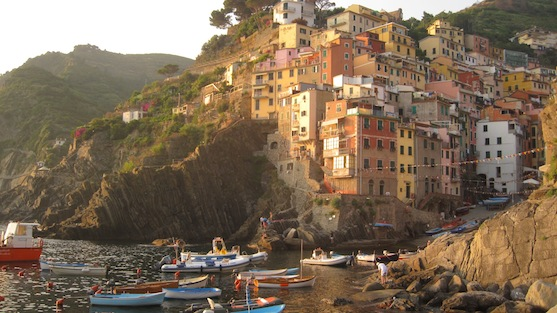
\includegraphics[width=0.8\textwidth]{figs/exercises/ex2/cinque_terre_small.jpg}
		}
		\caption{Before}
		\label{fig:ex2-before}
	\end{subfigure}%
	\begin{subfigure}{.5\textwidth}
		\centering
		\fbox{
			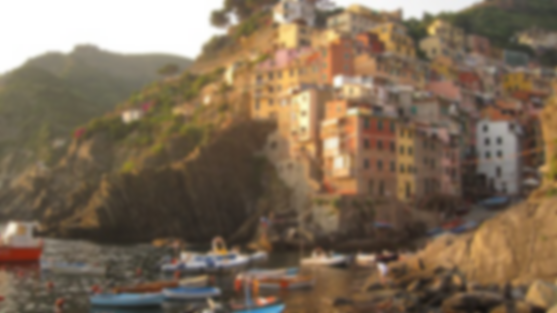
\includegraphics[width=0.8\textwidth]{figs/exercises/ex2/HW2_output.png}
		}
		\caption{After}
		\label{fig:ex2-after}
	\end{subfigure}
	\caption{Picture before and after blur effect is added}
	\label{fig:ex4}
\end{figure}

\begin{enumerate}
	\item[\textbf{Step 0}]

	\item[\textbf{Step 1}]

	\item[\textbf{Step 2}]

	\item[\textbf{Step 3}]
\end{enumerate}

\begin{figure}[ht]
	\centering
	\fbox{
		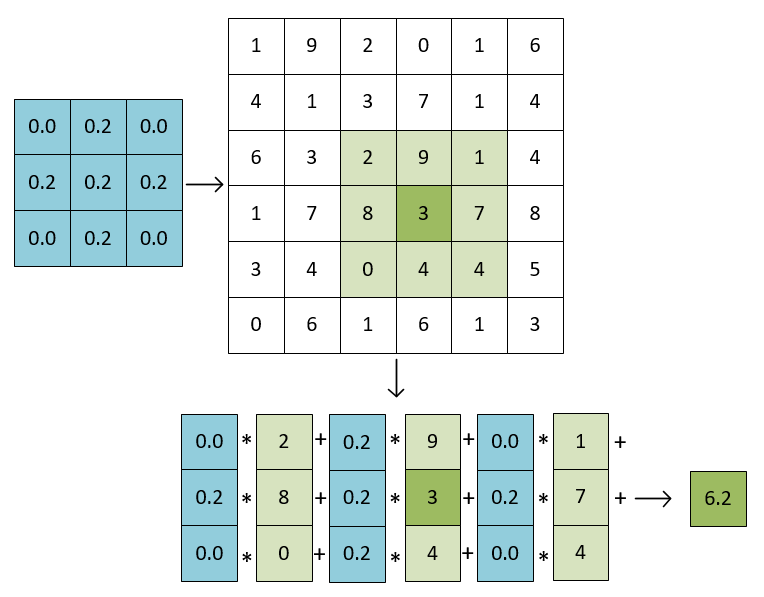
\includegraphics[width=0.8\textwidth]{figs/exercises/ex2/hw2.PNG}
	}
	\caption{TBD}
	\label{fig:ex2}
\end{figure}